\uuid{6995}
\titre{Exercice 6995}
\theme{}
\auteur{blanc-centi}
\date{2015/07/04}
\organisation{exo7}
\contenu{
  \texte{On considère l'équation différentielle
$$y'-e^xe^y=a$$
Déterminer ses solutions, en précisant soigneusement leurs intervalles de définition, pour}
\begin{enumerate}
  \item \question{$a=0$}
  \item \question{$a=-1$ (faire le changement de fonction inconnue $z(x)=x+y(x)$)}
\end{enumerate}
\begin{enumerate}
  \item \reponse{L'équation différentielle $y'-e^xe^y=0$ est à variables séparées: 
en effet, en divisant par $e^{y}$, on obtient $-y'e^{-y}=-e^x$. 
Le terme de gauche est la dérivée de $e^{-y}$ ($y$ est une fonction de $x$), 
celui de droite est la dérivée de $x\mapsto -e^x$: 
$$\frac{\dd e^{-y}}{\dd x} = \frac{\dd (-e^x)}{\dd x}$$
Les dérivées étant égales, cela implique que les deux fonctions sont égales à 
une constante additive près: ainsi $y$ est solution sur $I$ si et seulement si 
elle est dérivable sur $I$ et $\exists\,c\in\R,\ \forall x\in I$, $e^{-y}=-e^x+c$. 
\`A $c$ fixé, cette égalité n'est possible que si $-e^x+c>0$, 
c'est-à-dire si $c>0$ et $x<\ln c$. On obtient ainsi les solutions:
$$y_c(x)=-\ln(c-e^x)\quad (\text{pour } x\in I_c=]-\infty;\ln c[)$$
où $c$ est un paramètre réel strictement positif.

Pour que l'une des courbes intégrales passe par l'origine, il faut qu'il existe $c>0$ tel que $0\in I_c$ et $y_c(0)=0$: autrement dit, $c>1$ et $c-1=1$. Il s'agit donc de $y_2:x\mapsto-\ln(2-e^x)$, la courbe intégrale cherchée est son graphe, au-dessus de l'intervalle $I_2=]-\infty;\ln 2[$. Sa tangente en l'origine a pour pente $y_2'(0)=e^0e^{y(0)}=1$, c'est la première bissectrice. Comme par construction $y_2'$ est à valeurs strictement positives, la fonction $y_2$ est strictement croissante.

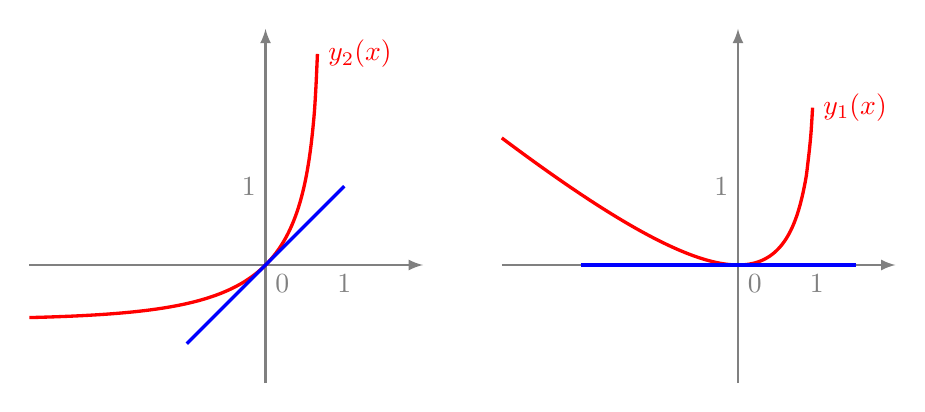
\begin{tikzpicture}[scale=1]

 \draw[->,>=latex,thick,gray] (-3,0)--(2,0);
 \draw[->,>=latex,thick,gray] (0,-1.5)--(0,+3);

 \draw [very thick, color=red,samples=200,smooth, domain=-3:0.66] plot(\x,{-ln(2-exp(\x))})
node[right]{$y_2(x)$};

\draw[very thick, blue] (-1,-1)--(+1,+1);

 \node[below right,gray] at (0,0) {$0$};
\node[below,gray] at (1,0) {$1$};
\node[left,gray] at (0,1) {$1$};


\begin{scope} [xshift=6cm]
 \draw[->,>=latex,thick,gray] (-3,0)--(2,0);
 \draw[->,>=latex,thick,gray] (0,-1.5)--(0,+3);

 \draw [very thick, color=red,samples=200,smooth, domain=-3:0.95] plot(\x,{-\x - ln(1-\x)})
node[right]{$y_1(x)$};

\draw[very thick, blue] (-2,0)--(+1.5,0);

 \node[below right,gray] at (0,0) {$0$};
\node[below,gray] at (1,0) {$1$};
\node[left,gray] at (0,1) {$1$};
\end{scope}

\end{tikzpicture}}
  \item \reponse{Posons $z(x)=x+y(x)$: $z$ a le m\^eme domaine de définition que $y$ et est dérivable 
si et seulement si $y$ l'est. En remplaçant $y(x)$ par $z(x)-x$ dans l'équation 
différentielle $y'-e^xe^y=-1$, on obtient $z'-e^z=0$, c'est-à-dire $z'e^{-z}=1$. 
Il s'agit de nouveau d'une équation à variables séparées: en intégrant cette égalité, 
on obtient que $z$ est solution sur $J$ si et seulement si elle est dérivable sur 
$J$ et $\exists\,c\in\R,\ \forall x\in J$, $e^{-z}=-x+c$. 
\`A $c$ fixé, cette égalité n'est possible que si $c>x$. On obtient ainsi les solutions:
$$y_c(x)=z_c(x)-x=-x-\ln(c-x)\quad (\text{pour } x\in J_c=]-\infty;c[)$$
où $c$ est un paramètre réel.

Pour que l'une des courbes intégrales passe par l'origine, 
il faut qu'il existe $c\in\R$ tel que $0\in J_c$ et $y_c(0)=0$: 
autrement dit, $c>0$ et $c=1$. Il s'agit donc de $y_1:x\mapsto-x-\ln(1-x)$, 
la courbe intégrale cherchée est son graphe, au-dessus de l'intervalle $J_1=]-\infty;1[$. 
Sa tangente en l'origine a pour pente $y_1'(0)=e^0e^{y(0)}-1=0$: elle est horizontale.}
\end{enumerate}
}